\documentclass[sigplan,screen,10pt]{acmart}
\usepackage[utf8]{inputenc}
\usepackage{amsmath}
\usepackage{amsfonts}
%\usepackage{amssymb}
\usepackage{amsthm}
\usepackage{graphicx}
%\usepackage{xcolor}
%\usepackage{soul}
%\usepackage{hyperref}
\usepackage{algorithm}
\usepackage[noend]{algpseudocode}
%\usepackage{dsfont}
%\usepackage[font=small, labelfont=bf]{caption}
%\usepackage[left=2cm,right=2cm,top=2cm,bottom=2cm]{geometry}
\usepackage{subcaption}
\usepackage{todonotes}
\usepackage{multirow}
\newcommand\el[1]{\textcolor{orange}{{\bf Erick: }#1}}

\newcommand\ssbtokens[0]{\textit{SSB-Tokens} }
\newcommand\invpathcomment[0]{ \Statex \Comment{{\color{commentgray}On \textit{msg}; properties (in italics) without an explicit access path belong to \textit{msg.content}.}}}

\definecolor{commentgray}{gray}{0.40}

\hyphenation{block-chain}
\hyphenation{block-chains}
\hyphenation{Ethe-reum}


\copyrightyear{2022} 
\acmYear{2022} 
\setcopyright{rightsretained} 

\renewcommand{\copyrightpermissionfootnoterule}{%
\hrule
 \vspace*{-2pt}
  \noindent%
\\
\hfill
  
\includegraphics[width=0.20\columnwidth]{creative-commons-by_sa_4_0}
 \hfill
  \begin{minipage}[b]{0.75\columnwidth}
    \footnotesize 

This work is licensed under a \href{http://creativecommons.org/licenses/by-sa/4.0/}{Creative Commons Attribution-ShareAlike International 4.0 License}.
  \end{minipage}%
  \vspace*{2pt}%
\hrule
  \vspace*{2pt}
}


\acmConference[DICG'22]{3rd International Workshop on Distributed Infrastructure for Common Good}{Dec.  2022}{Montreal, Quebec, Canada}
\acmBooktitle{3rd International Workshop on Distributed Infrastructure for Common Good (DICG'22), December 2022, Montreal, Quebec, Canada}\acmDOI{XXX}
\acmISBN{XXX-X-XXXX-XXXX-X/XX/XX}

\begin{CCSXML}
<ccs2012>
   <concept>
       <concept_id>10010520.10010521.10010537.10010540</concept_id>
       <concept_desc>Computer systems organization~Peer-to-peer architectures</concept_desc>
       <concept_significance>500</concept_significance>
       </concept>
 </ccs2012>
\end{CCSXML}

\ccsdesc[500]{Computer systems organization ~Peer-to-peer architectures}

\keywords{economics, peer-to-peer, crypto-tokens, blockchain, local economies, producer credit, gossip algorithms}

\begin{document}


\title{SSB-Tokens: Efficient Secure Asset Gossip for Trust-Based Local Economics}

\author{Erick Lavoie}
\email{erick.lavoie@unibas.ch}
\affiliation{%
  \institution{University of Basel, Basel, Switzerland}
}

\author{Christian Tschudin}
\email{christian.tschudin@unibas.ch}
\affiliation{%
  \institution{University of Basel, Basel, Switzerland}
}


\begin{abstract}

\end{abstract}

\maketitle

\section{Introduction}

Major blockchain projects, such as Bitcoin (CITE) and Ethereum (CITE), implement \textit{global financial infrastructure}, respectively as a replicated ledger or as a state-machine. In both cases, creating new tokens, by forking an existing project or implementing them as smart-contracts, requires specialized technical skills. Moreover, maintaining the integrity of transactions demands Internet connectivity, and requires significant energy (CITE) or capital investment (CITE). The resulting costs become prohibitive for many applications that are inherently \textit{local} to a region or community.

For those applications, we propose instead to \textit{localize} the operations of crypto-token infrastructure in multiple complementary ways based on the following insights: (1) The creation of tokens is done by specific identities and authenticated, preventing any other identity to forge tokens for a different identity, foregoing the need for a global mining process; (2) The value of each specific token derives from the trust that its individual creator will fulfill the obligations they have linked to the tokens, instead of speculation on the future demand of a single token fuelled by artificial scarcity in its total supply; (3) Transactions are public to a \textit{local} community, e.g. linked to a geographical region or bound by common interest, and recorded on identity-specific (immutable) append-only logs, instead of globally shared on a single global ledger; (4) Verification of the integrity of operations is done by each participant for the operations on which they depend, instead of having specialized miners performing the verification tasks for others; and, (5) Proofs of fraud are immutable, linked to a specific identity, and the cost of fraud is ultimately the exclusion of that identity from participation in a community, which can be a greater loss than the potential gains obtained from fraud on common transactions, incentivizing correct behavior. Compared to Bitcoin or Ethereum-based alternatives, localizing the operations simplifies the implementation of crypto-tokens and removes much of the technical or capital costs of maintaining transaction integrity. Instead our approach replaces technical complexity and capital stakes with social trust and reputation, yet still enables a large variety of applications to be supported.

The main remaining technical challenge is to efficiently validate past operations, i.e. ensuring that tokens were not spent more than once prior to giving them to other users. To do so, each user is responsible for validating both the format and the availability of tokens they receive from others. 
%When validation fails, users can flag the incorrect transactions to remember and report them to others. Users that wrongly flag the transactions of others can be blocked from replication using the existing core operations of SSB and therefore excluded from future transactions. ß
As validity depends on an ever growing chain of transactions, we avoid verifying the same operations more than once by establishing a \textit{verification frontier} up to which all operations from a given user have been locally validated, effectively leveraging the \textit{total order} provided by append-only logs of Secure-Scuttlebutt (CITE). Using a validation frontier instead of an explicit index of valid transactions lowers memory requirements.

%TODO: Discuss the benefits and challenges of using append-only logs for recording transactions. E.g. a log fork currently results in a partitioning of the SSB network, with implementations refusing to carry updates from the fork they do not carry. A proof-of-fork is recorded by publishing a message that links to both messages with the same sequence number. Because a user cryptographically signs their message, this acts as a proof of misbehaviour. For cases where the stakes are high enough to require proving that there are enough remaining tokens \textit{prior to the transaction}, a third trusted party can act as a \textit{witness}. Most commonly, the creator of the tokens has the incentive to do this but any other user can also do it.

In this paper, we build on the previous insights to present \textit{an efficient system for secure asset gossip built on top of Secure-Scuttlebutt}. Specifically:
\begin{itemize}
 \item We present the design and implementation of \ssbtokens, a new crypto-token infrastructure that enables any user to securely issue their own tokens, send tokens to others, and flag invalid transactions, as well as efficiently validate previous operations through a \textit{validation frontier};
 \item  We present diverse applications that can be implemented with \ssbtokens including fidelity cards, open source contribution tracking, crowdfunding of local projects, and token-supported mesh networking, showing the generality of our design;
 \item We show that our implementation can run on affordable hardware, such as Raspberry Pis. We test our system on real-world traces of transactions from ERC tokens showing that our implementation can support similar number of transactions and users, at reasonable processing time and storage.
\end{itemize}

In the rest of this paper,  we present the design of \ssbtokens (Section~\ref{section:design}), we present a variety of applications supported (Section~\ref{section:applications}), we evaluate the implementation on real-world transaction traces (Section~\ref{section:evaluation}), we compare to related projects (Section~\ref{section:related-work}) and finally conclude with future research directions (Section~\ref{section:conclusion}).




\section{SSB-Tokens}
\label{section:design}

In this section, we present our design first by establishing the system model on which it is built, which we inherit from Secure-Scuttlebutt. We then present the message format for all core operations of \ssbtokens and discuss the associated operations. We then make explicit the expected invariants on message values both to validate inputs prior to creating new messages and also to identify incorrect messages that might be produced by malicious actors. We follow with the core algorithms required to compute the unspent tokens received from specific operations and the overall balance of a specific token for any given owner, as well as an incremental algorithm to perform validation of past operations. This forms a complete design that could be implemented in many languages and for other communication infrastructure with similar characteristics as Secure-Scuttlebutt.

\subsection{System Model}

First, we assume a fully asynchronous environment between any two nodes, i.e. that a message created by a node may take an arbitrary long time before being replicated on any other node. We further assume any message will eventually be replicated.\footnote{The implementation of SSB requires a stronger assumption for synchronization between a pair of temporarily-connected replicas: it actually relies on partial synchrony, i.e. that most messages will be delivered before a timeout between two nodes. However, it may take an arbitrary long time for any two pair of nodes to contact and connect to each other to replicate messages, therefore from an application perspective the infrastructure operates in an asynchronous environment.}

Second, every node has an identity that corresponds to the public key of the public-private key pair that is used for signing messages, which guarantees that messages cannot be forged by nodes that don't have access to the corresponding private key. Messages are organized in an append-only log, i.e. an immutable list that can only be extended but never updated, linked to a single identity. These two properties are provided by the underlying SSB implementation~\cite{kermarrec2020gossiping}.

Third, we assume that every node has enough storage to replicate all messages from other nodes within their community. As shown in Section~\ref{section:storage}, current common devices can store messages from \el{Empirical number X}s of users, which should be sufficient for most local applications.

Fourth, for presentation simplicity, we assume a single node and its identity correspond to a single physical person and that all activity of that person are recorded on the same log. However, in practice, implementations may allow different applications for the same person to segregate their messages in different logs without loss of generality. A log may also be updated following synchronization between different physical persons through an out-of-band protocol so that the log may represent a collective identity,  but this is out-of-scope of this paper and not covered by SSB's core operations at the time of writing.

\subsection{Message Format and Semantics}

\begin{figure}[t]
\flushleft
\texttt{ msg = \{ 
     "key": \textbf{SSBMsgId}
     "author": \textbf{SSBLogId}, 
     "sequence": \textbf{Number}, 
     "previous": \textbf{SSBMsgId} || \textbf{null},  
     "content": \textbf{Object},
     "signature": \textbf{String}
\} 
     }
\caption[]{SSB message schema (JSON notation augmented with types in bold). Application messages are stored in \textit{msg.content}.\footnotemark }
\label{fig:ssb-message-schema}
\end{figure}

\footnotetext{This is a simplified (two-level) schema to improve the readability of algoritms. The actual SSB JavaScript implementation instead uses three levels: \textit{msg.key} is on the first level; all other properties are on a second level under \textit{msg.value}; and the application content is on the third level under \textit{msg.value.content}. The three levels make it clearer that the key to identify a message is derived from the content of \textit{msg.value} but introduce unnecessary verbosity when presenting our algorithms.}

All our messages are stored as content of SSB messages (Figure~\ref{fig:ssb-message-schema}). Notably, for a given message \textit{msg}, its identifier is accessible through \textit{msg.key}, its author as \textit{msg.author}, its sequence number as \textit{msg.sequence}, its ancestor in the log as \textit{msg.previous}, and its content as \textit{msg.content}.


\begin{table*}[t]
\centering
\caption{Message format of \ssbtokens operations (JSON notation augmented with types in bold), stored in \textit{msg.content} of a SSB Message.}
\label{table:api}
\begin{tabular}{|l|l|} 
\hline
\textbf{Message Types}          & \textbf{Semantics}                                                                                                           \\ 
\hline
\begin{tabular}{@{}l@{}}
\texttt{\{ "type": "tokens/create", "amount": \textbf{Number},}  \\
\texttt{"name": \textbf{String}, "unit": \textbf{String}, "description": \textbf{SSBMsgId} } \\ 
 \texttt{"smallest-unit": \textbf{Number}, "tokenHash": \textbf{String} \}}
\end{tabular} ~& 
\begin{tabular}{@{}l@{}}Create \textit{amount} tokens identified by \textit{name} \\ denominated in \textit{units}, with minimum \\ 
sub-division of \textit{smallest-unit}, binding creator to \\
 promises in \textit{description}. \end{tabular}                                  \\ 
\hline
\begin{tabular}{@{}l@{}}
\texttt{\{ "type": "tokens/give", "sources": [ \{ "amount": \textbf{Number},} \\
\texttt{ "id": \textbf{SSBMsgId} \}, ... ], "receiver": \textbf{SSBLogId}, } \\
\texttt{"amount": \textbf{Number}, "tokenHash":  \textbf{String} \}}     
\end{tabular}
& Give \textit{amount} tokens from \textit{sources} to \textit{receiver}.                                                                 \\ 
\hline
\begin{tabular}{@{}l@{}}
\texttt{\{ "type": "tokens/burn", "sources" : [ \textbf{SSBMsgId}, ... ] } \\
\texttt{"amount": \textbf{Number}, "tokenHash": \textbf{String} \}}    
\end{tabular}             & Destroy tokens from \textit{sources}.                                                                                             \\ 
\hline
\begin{tabular}{@{}l@{}}
\texttt{\{ "type": "tokens/flag", "sources": [ \textbf{SSBMsgId}, ... ],} \\
 \texttt{ "label": \textbf{String}, "tokenHash": \textbf{String} \}} 
 \end{tabular}      &  
 \begin{tabular}{@{}l@{}}
 Assign a flag with \textit{label} on \textit{sources}. \\
 \end{tabular}                             \\ 
\hline
\begin{tabular}{@{}l@{}}
\texttt{\{ "type": "tokens/unflag", "flag": \textbf{SSBMsgId} \}}    
\end{tabular}
 & \begin{tabular}{@{}l@{}}Remove a previously assigned \textit{flag}.  \end{tabular}                               \\ 
\hline
%\texttt{list(tokenHash :String, owner :SSBLogId)}          & \begin{tabular}{@{}l@{}}List the current state of token, identified \\ by \textit{tokenHash}, owned by \textit{owner}.   \end{tabular}                             \\ 
%\hline
%\texttt{validate(amount :Number, src :SSBMsgId)}    & \begin{tabular}{@{}l@{}}Validate that \textit{src} has \textit{amount} \\ available and all transitive sources are valid. \end{tabular}  \\
%\hline
\end{tabular}
\end{table*}

All of \ssbtokens operations, performed by users, have corresponding messages to store them in logs. We use interchangeably \textit{operations} and \textit{messages} to refer to them, the context makes it clear whether we specifically refer to the action performed by users or its persisted record as a message in a log. All operations are stored as the \textit{content} of SSB messages. Operations also reuse some of the fields of SSB messages to avoid redundancy: their \textit{identifier} and \textit{author} are the same as the identifier and author of SSB messages that contains them.\footnote{The application programming interface of \ssbtokens assigns both properties respectively as \textit{id} and \textit{author} of objects representing the operations, to abstract the underlying SSB storage format.}

Table~\ref{table:api} shows the syntactic message format of \ssbtokens and their associated semantics. The core of \ssbtokens is organized around \texttt{create}, an operation that creates a certain number of tokens, associated specifically to their creator; \texttt{give}, an operation to transfer a subset of tokens from one or multiple sources to another user; and \texttt{burn} an operation to destroy all tokens from a given (owned) source, for example, when another user has redeemed the real-world underlying value represented by the token.  Note that the give operation is unilateral, i.e. it does not require acceptance by the recipient to be effective. In case a recipient receives tokens they did not want, they can block the sender or burn the tokens. Notice also that a \texttt{burn} should destroy the entire original amount of tokens in their sources. This simplifies reasoning about tokens flows, as only the \texttt{give} operation can split a source into many. Shall a partial burn be need, a user can first give a partial amount of a source to themselves then burn the new give operation.

In addition to the core operations for manipulating tokens, the \texttt{flag} and \texttt{unflag} enables users to assign labels to recorded operations. This can be useful for example to share that a user found invalid messages in other logs, or to enable the creator to cancel tokens that are circulating, or ask their owners to return them in exchange for newer valid tokens. The validation of past operations (Alg.~\ref{algorithm:validation}) does not rely on flags, only the format and values of messages for core operations to prevent malicious users from tempering with the validation process. However, the labels may still alert other users to invalid operations and focus their validation efforts on those first to verify for themselves that they were indeed invalid. After a second validation that was inconsistent with the flags applied by malicious users, a user may decide to block the authors of invalid flags using the core operations of SSB~\cite{kermarrec2020gossiping}. The label of flags is user-defined enabling users to find additional uses beyond the two precendent.

% The \texttt{flag} and \texttt{unflag} operations are used for multiple uses. First, the creator of the tokens can \textit{cancel} tokens in circulation that have not yet been returned, to signify that the associated promise won't be honored. Second, receivers of invalid tokens, e.g. they were incorrectly formatted or the associated source did not have a sufficient remaining balance, can report the incorrect operations to exclude them from available funds locally and warn others that the operations may be incorrect. In addition, the \textit{label} field is user-defined to enable other potential user applications.

In addition, to their specific fields, all messages (but \texttt{unflag}) include an  an additional \textit{tokenHash} property. The \textit{tokenHash} makes it faster to query for all messages specific to a given token, without having to first retrieve the corresponding \texttt{create} messages through a transitive list of sources. As shown later in the invariants of a \texttt{create} operation (Alg.~\ref{alg:create}), the \textit{tokenHash} combines all attributes of the token (name, unit, description, and smallest unit) with its author, making the hash (and identity) of a token specific to an author and unique among all tokens.

\subsection{Invariants}

In this section, we make explicit all the invariants assumed on the messages for them to be considered valid. The list of invariants is used for two purposes: first to validate user inputs as part of the API prior to publishing corresponding messages on SSB, and, second, to validate messages published by other users, as we have no guarantee that their implementation of \ssbtokens actually implements the expected invariants and algorithms.

The \texttt{create} operation invariants (Alg.~\ref{alg:create}) are actually the simplest. Invariant~\ref{alg:create}.\ref{alg:create:positive-amount} requires the number of created tokens to be positive, which prevents pollution of the database with unnecessary null or negative "creations". Invariant~\ref{alg:create}.\ref{alg:create:unique-hash} ensures the \textit{tokenHash} will be unique for every combination of token properties and author, speeding the identification of relevant messages in the local store. It also ensures the hash is unforgeable, because only the correct \textit{author} can sign messages in which the author used for the \textit{tokenHash} is coherent with the SSB \textit{msg.author}. The token properties also only appear on a creation message, every other message refer to the properties using the \textit{tokenHash} instead.

\begin{algorithm}
\begin{algorithmic}[1]
\invpathcomment
  \State \textbf{Positive amount:} $\textit{amount} > 0$ \label{alg:create:positive-amount}
  \State \textbf{Unique unforgeable token identifier:} \newline $\textit{tokenHash} = \texttt{hash}(\textit{msg.author} \oplus \textit{name} \oplus \textit{unit} \oplus  \textit{description} \oplus 
                                                                    \textit{smallest-unit})$ \label{alg:create:unique-hash}
\end{algorithmic}
\caption{\texttt{Create} operation invariants}
\label{alg:create}
\end{algorithm}

The \texttt{give} operation invariants (Alg.~\ref{alg:give}) are the most numerous and subtle but follow naturally from the structure of the messages.

\begin{algorithm}
\begin{algorithmic}[1]
\invpathcomment
  \State \textbf{Bounded sources}: Number of \textit{sources} is less or equal to 10.
  \State \textbf{Valid sources}: For each \textit{src} in \textit{sources}, \textit{src.id} references either a message with type \texttt{"tokens/create"} or \texttt{"tokens/give"}
  \State \textbf{Unique sources}: For each \textit{src} in \textit{sources}, \textit{src.id} is unique among all \textit{sources}
  \State \textbf{Consistent tokenHash}: For each \textit{src} in \textit{sources}, \textit{src.id}'s message \textit{tokenHash} is equal to \textit{tokenHash}
  \State \textbf{Positive amounts}: For each \textit{src} in \textit{sources}, \textit{src.amount} is greater than $0$
  \State \textbf{Available funds}: For each \textit{src} in \textit{sources} and \textit{msg'} such that \textit{msg'.key = src.id}, \textit{src.amount} is smaller or equal to the unspent balance of \textit{msg'} up to \textit{msg.sequence} of \textit{msg.author} (Alg.~\ref{alg:unspent})
  \State \textbf{Divisible sources}: For each \textit{src} in \textit{sources}, \textit{src.amount} is a multiple of \textit{smallest-unit} of the root of \textit{src.id}
  \State \textbf{Consistent amounts}: The sum of all \textit{src.amount} in \textit{sources} is equal to \textit{amount}
  \State \textbf{Consistent creator}: If \textit{msg'} with type \texttt{tokens/create} exists such that \textit{msg' .key = src.id} in \textit{sources}, \textit{msg'.author = msg.author}
  \State \textbf{Consistent recipient}: If \textit{msg'} with type \texttt{tokens/give} exists such that \textit{msg'.key = src.id} in \textit{sources}, \textit{msg'.content.recipient = msg.author}
\end{algorithmic}
\caption{\texttt{Give} operation invariants}
\label{alg:give}
\end{algorithm}

\begin{algorithm}
\begin{algorithmic}[1]
\invpathcomment
  \State Number of \textit{sources} is less or equal to 10.
  \State For each \textit{msg'} referred by key \textit{id} in \textit{sources}, \textit{msg'.content.type} is equal to \texttt{"tokens/create"} or \texttt{"tokens/give"}
  \State For each \textit{msg'} referred by key \textit{id} in \textit{sources}, \textit{msg'.key} is unique among all \textit{sources}
  \State For each \textit{msg'} referred by key \textit{id} in \textit{sources}, \textit{msg'.content.tokenHash} is equal to \textit{tokenHash}
  \State For each \textit{msg'} referred by key \textit{id} in \textit{sources}, none of the funds have been spent: the unspent amount of \textit{msg'} up to \textit{msg.sequence} of \textit{msg.author} is equal to \textit{msg'.content.amount} (Alg.~\ref{alg:unspent}).
\end{algorithmic}
\caption{\texttt{Burn} operation invariants.}
\label{alg:burn}
\end{algorithm}

\begin{algorithm}
\begin{algorithmic}[1]
\invpathcomment
  \State Number of \textit{sources} is less or equal to 10.
   \State For each \textit{msg'} referred by key \textit{id} in \textit{sources}, \textit{msg'.content.tokenHash} is equal to \textit{tokenHash}
\end{algorithmic}
\caption{\texttt{Flag} operation invariants.}
\label{alg:flag}
\end{algorithm}

\subsection{Computing Balances}

\begin{algorithm}
\caption{\texttt{unspent(msg, owner, seqno)}: Computing the number of unspent tokens of an operation recorded in \textit{msg}, up to \textit{seqno} of \textit{owner}'s log. \textit{owner} must be the creator or recipient of the tokens in \textit{msg}.}
\label{alg:unspent}
\begin{algorithmic}[1]
  \State \textit{type'} $\leftarrow$ \textit{msg'.content.type}
  \State \textit{SrcTypes} $\leftarrow \{ \texttt{"tokens/create"}, \texttt{"tokens/give"} \}$
  \If{$\textit{type} \notin \textit{SrcTypes}$} \textbf{Error}
  \EndIf
  \If{$\textit{type} = \texttt{"tokens/create"}$}
      \If {$\textit{msg.author} \neq \textit{owner}$} \textbf{Error}
      \EndIf
  \EndIf
  \If{$\textit{type} = \texttt{"tokens/give"}$}
      \If {$\textit{msg.content.recipient} \neq \textit{owner}$} \textbf{Error}
      \EndIf
  \EndIf
  \State
    \State \textit{amnt} $\leftarrow$ \textit{msg.content.amount}
    \For{\textit{msg'} ~\textbf{in}~ all messages \textbf{from} \textit{owner}}
        \State \textit{type'} $\leftarrow$ \textit{msg'.content.type}
        \If{ $\textit{msg'.sequence} <= \textit{seqno}$}
            \If{\textit{type'} $= \texttt{"tokens/give"}$}
                \For{\textit{src'} \textbf{in} \textit{msg'.content.sources}}
            	    \If{$\textit{msg.key} = src'.id$} 
	                  \State  $\textit{amnt} \leftarrow \textit{amnt} - \textit{src'.amount}$
	             \EndIf
                \EndFor
            \ElsIf{\textit{type'} $= \texttt{"tokens/burn"}$}
                \For{\textit{id'} \textbf{in} \textit{msg'.content.sources}}
            	    \If{$\textit{msg.key} = id'$} 
	                  \State  $\textit{amnt} \leftarrow \textit{amnt} - \texttt{get}(\textit{src'})\textit{.amount}$
	             \EndIf
                \EndFor 
            \EndIf
        \EndIf 
    \EndFor
  \State \Return \textit{amnt}
\end{algorithmic}
\label{alg:unspent}
\end{algorithm}

\begin{algorithm}
\begin{algorithmic}[1]
  \State \textbf{Require:} 
  \begin{itemize}
    \item a function \texttt{get}(\textit{ssbMsgId}) that returns an SSB msg from the local store if it exists, null otherwise;
    \item that local messages have been validated first (Alg.~\ref{alg:validation}).
  \end{itemize}
  \State
  \State \textit{Create} $\leftarrow$ \texttt{"tokens/create"}
  \State \textit{Give} $\leftarrow$ \texttt{"tokens/give"}
  \State \textit{Burn} $\leftarrow$ \texttt{"tokens/burn"}
  \State \textit{Ops} $\leftarrow$ \{ Create, Give, Burn \}
  \State
  \State $\textit{bal} \leftarrow 0$
  \For{\textit{msg'} \textbf{in} all valid local messages}
      \State \textit{type'} $\leftarrow$ \textit{msg'.content.type}
      \If{\textit{type'} $\notin \textit{Ops}$} \textbf{continue}
      \EndIf

   \State
    \State \textit{tokenHash'} $\leftarrow$ \textit{msg'.content.tokenHash}
    \If{ \textit{tokenHash'} $\neq tokenHash$ }  \textbf{continue}
    \EndIf
    \State
    \State \textit{author'} $\leftarrow$ \textit{msg'.author}
    \If{$\textit{type'} = \texttt{Create}$ ~\textbf{and}~ 
        $\textit{author'} = \textit{owner}$
        }
    	\State $\textit{bal} \leftarrow \textit{bal} + \textit{msg'.content.amount}$
   \ElsIf{$\textit{type'} = \textit{Give}$}
        \If{$\textit{msg'.content.recipient} = \textit{owner}$} 
             \State $\textit{bal} \leftarrow \textit{bal} + \textit{msg'.content.amount}$
        \EndIf
         \If{$\textit{author'} = \textit{owner}$} 
             \For{\textit{src} ~\textbf{in}~ \textit{msg'.content.sources}}
                 \State $\textit{bal} \leftarrow \textit{bal} - \textit{src.amount}$    
             \EndFor    
        \EndIf
   \ElsIf{$\textit{type'} = \texttt{Burn}$ ~\textbf{and}~ 
        $\textit{author'} = \textit{owner}$}
         \For{\textit{src} ~\textbf{in}~ \textit{msg'.content.sources}}
             \State $\textit{bal} \leftarrow \textit{bal} - \texttt{get}(\textit{src).amount}$    
         \EndFor    
    \EndIf
  \EndFor
  \State \Return \textit{bal}
\end{algorithmic}
\caption{\texttt{balance(tokenHash, owner)}: Computing the balance of a token, uniquely defined by \textit{tokenHash}, for \textit{owner}.}
\label{alg:balance}
\end{algorithm}

\subsection{Validating Operations}

Validation frontier: (log id, seq no, last op message id)

\begin{algorithm}
\begin{algorithmic}[1]
  \Statex \textbf{Require:} 
  \begin{itemize}
    \item a function \texttt{forkNo}(\textit{author}) that returns the earliest \textit{seqno} for which we have a proof of a fork of \textit{author}'s log, $\infty$ if none; 
    \item a function \texttt{get}(\textit{ssbMsgId}) that returns an SSB Msg from the local store if it exists, null otherwise.
  \end{itemize}
  \State 
  \State \textit{invalid} $\leftarrow \{ \}$ \Comment{Set of SSBMsgId}
  \State \textit{frontier} $\leftarrow \{ \}$  \Comment{Dict.  of SSBLogId -> SSBMsg}
  \State \Comment{"tokens/" replaced by "./" for brevity}
  \State \textit{Ops} $\leftarrow \{ \texttt{"./create"}, \texttt{"./give"}, \texttt{"./burn"}, \texttt{"./flag"} \}$
  \State
   \Procedure{valid}{\textit{msg}}
      \State $\textit{author} \leftarrow \textit{msg.author}$
       \State $\textit{seqno} \leftarrow \textit{msg.sequence}$
       \State $\textit{id} \leftarrow \textit{msg.key}$
       \State $\textit{type} \leftarrow \textit{msg.content.type}$
       \State $\textit{tip} \leftarrow \textit{frontier[msg.author]}$       
       \State $\textit{tipNo} \leftarrow \textit{frontier}\textit{[msg.author].sequence}$
       \State $\textit{ops} \leftarrow $ token ops from \textit{author} within [\textit{tipNo}, \textit{seqno}[
       \State
       \If{$\textit{type} \notin \textit{Ops}$} \Return \textbf{false}
       
      \ElsIf{$\textit{msg.key} \in invalid$} \Return \textbf{false}
      \ElsIf{$\textit{seqno} \geq \textit{forkNo(author)}$} \Return \textbf{false}
      \ElsIf{$\textit{msg} \text{ log ancestor of } \textit{tip}$} 
          \State \Return \textbf{true}
      \ElsIf{\textit{tip} is \textbf{not} a log ancestor of \textit{msg}}
          \State \Return \textbf{false}
      \EndIf

     \State
      \State \textit{srcsOk} $\leftarrow \textbf{true}$       \Comment{Check all sources and message}
      \If{\textit{msg.content} has \textit{sources}}
      	\For{$\textit{src} ~\textbf{in}~ \textit{msg.content.sources}$}
	   \If{$\textit{type} = \texttt{"tokens/create"}$}
	     \State $\textit{src} \leftarrow \textit{src.id}$
	   \EndIf
	    \State \textit{srcsOk} $\leftarrow \textit{srcsOk} ~\textbf{and}~  \texttt{valid}(\texttt{get}(\textit{src}))$
           \EndFor
       \EndIf
       \State
       \If{invariants on \textit{msg} are ok \textbf{and} \textit{srcsOk}}
          \If{$ops \subseteq \textit{invalid}$} \Comment{Includes $\textit{ops} = \emptyset$}
              \State $\textit{frontier[author]} \leftarrow \textit{msg}$
          \EndIf
           \State \Return \textbf{true}
       \Else
            \State $\textit{invalid} \leftarrow \textit{invalid} \cup \{ id \}$
            \State \Return \textbf{false}
       \EndIf
   \EndProcedure
\end{algorithmic}
\caption{Validation of token operations with caching.}
\label{alg:validation}
\end{algorithm}

Incremental validation of operations can be performed with a topological sorting of all operations and calling \texttt{valid} from the earliest to the latest.


Possible optimizations: 
\begin{itemize}
    \item Once the number of invalid operations for an author is larger than a predefined bound, the author can be blocked and all operations considered invalid.
\end{itemize}

In case a fork is detected, all downstream operations of operations that have happened after the fork should be invalidated. A fork may happen after an arbitrary long time, there exists no time after which we are guaranteed to not detect a fork.

\subsubsection{Double-Spending}


\begin{figure}[hb]
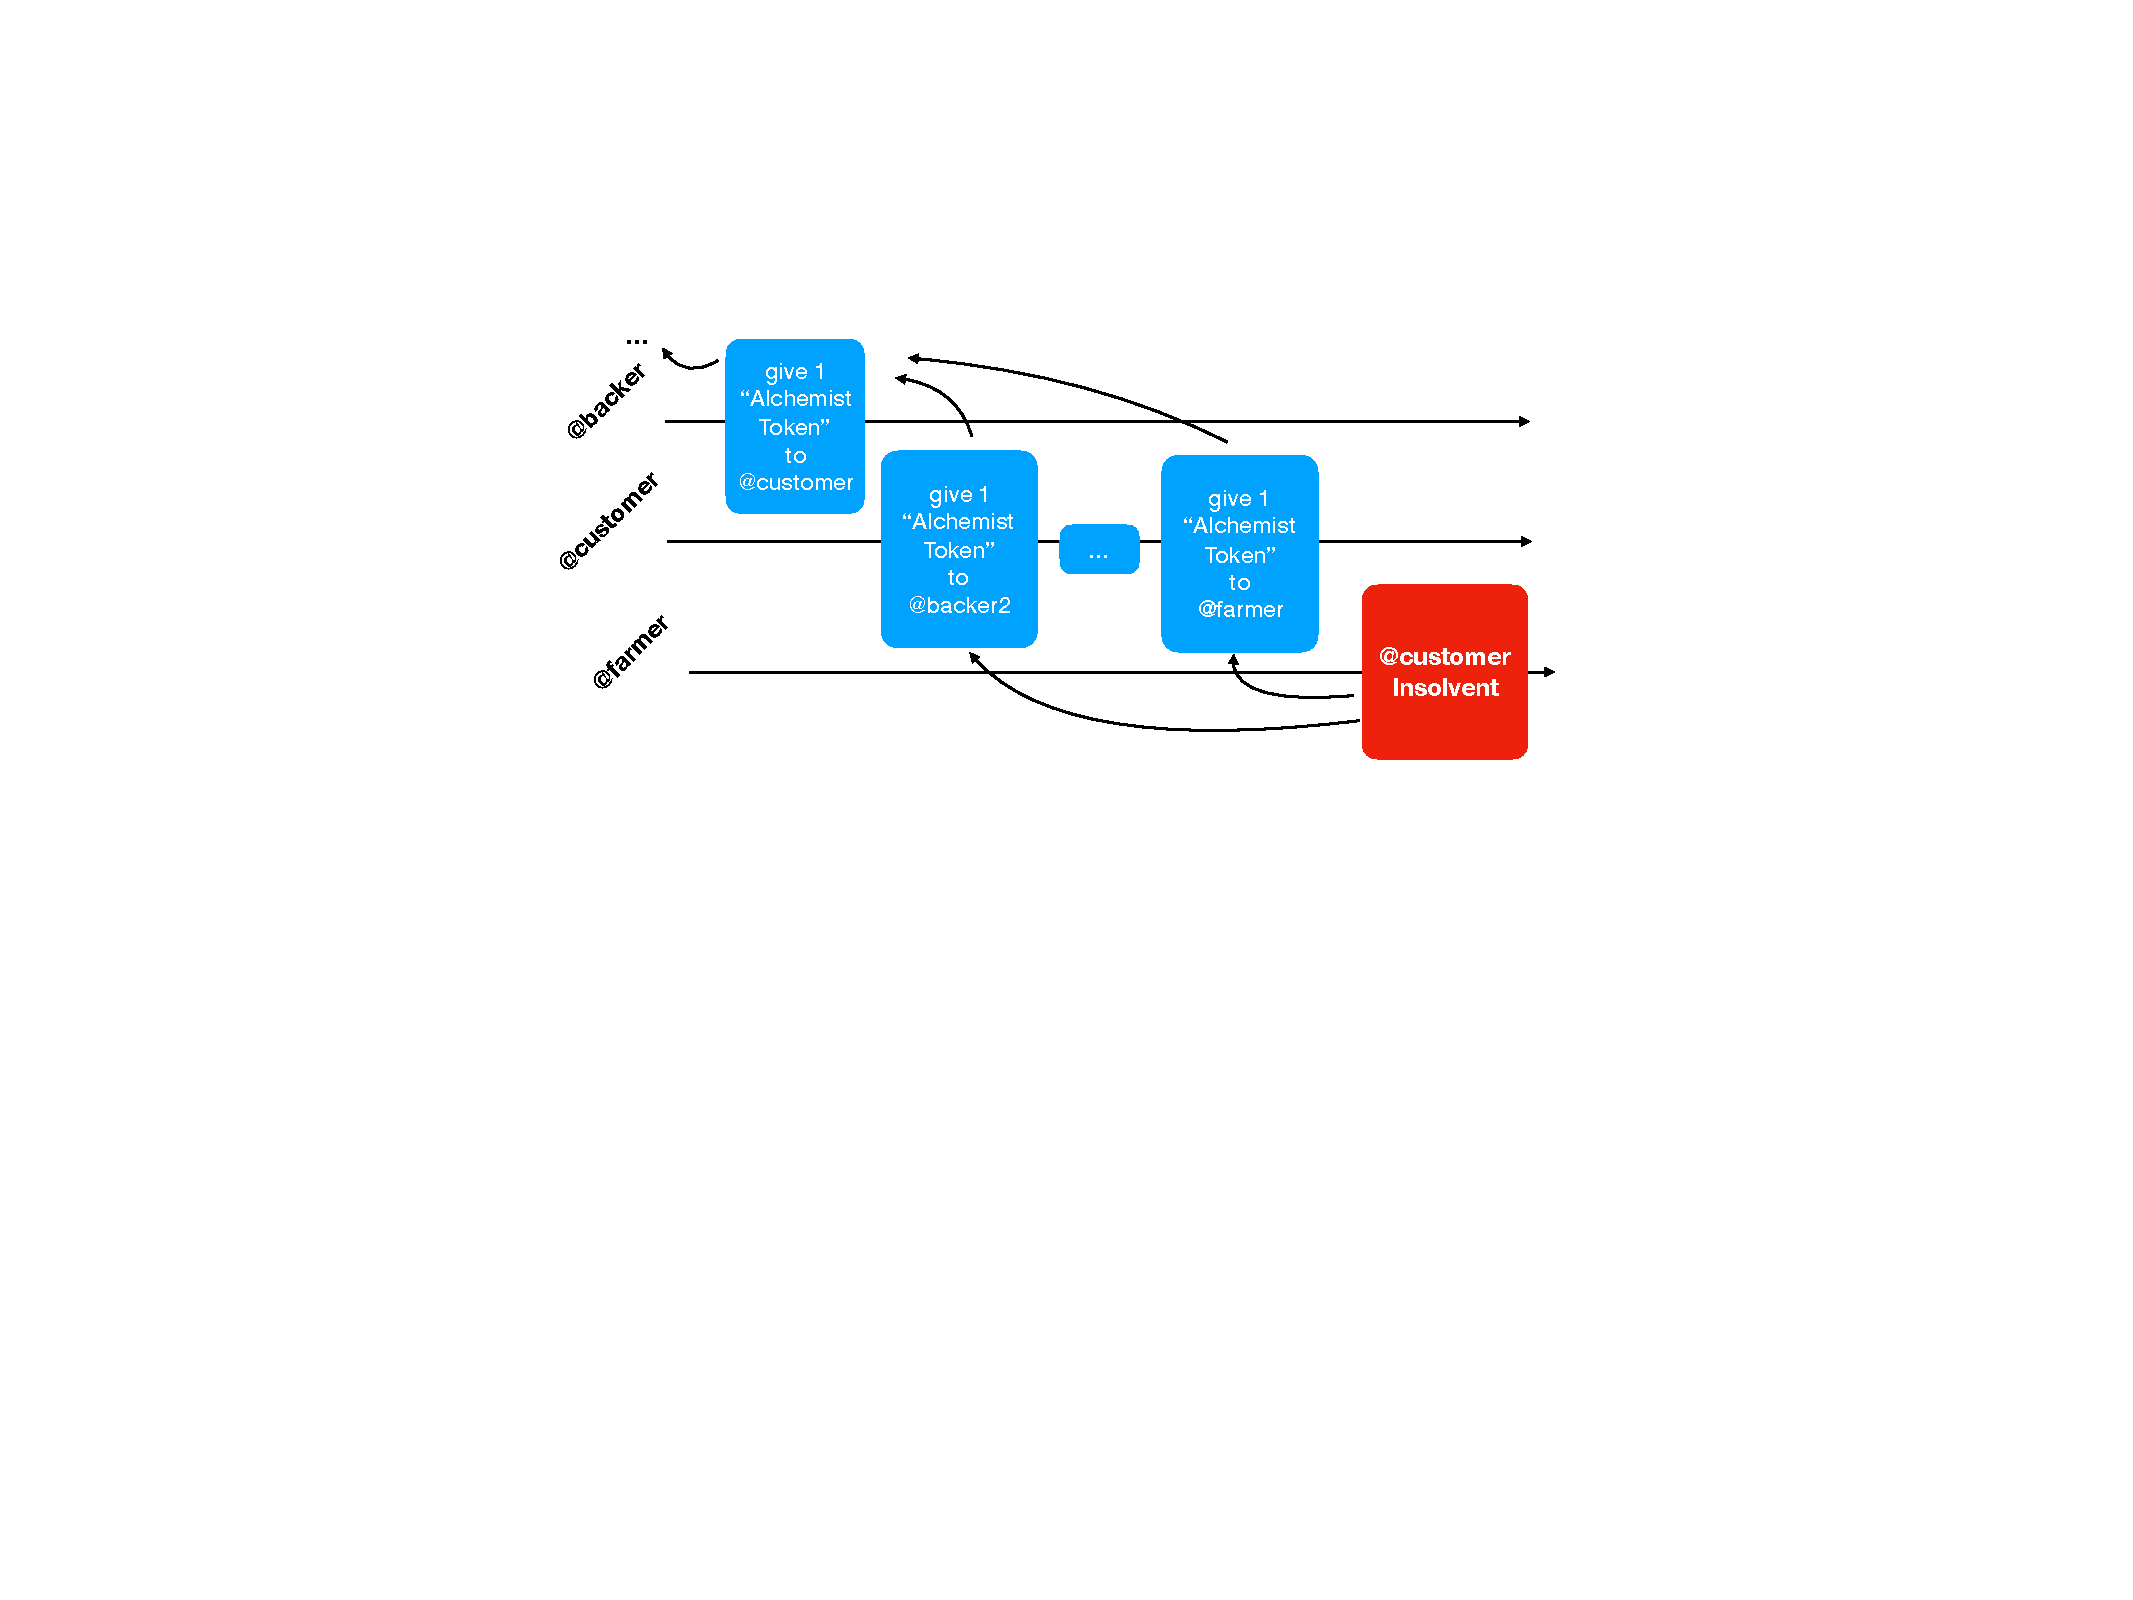
\includegraphics[width=0.45\textwidth]{figures/double-spend}
\caption{Double-Spend}
\end{figure}


\begin{figure}[hb]
\centering
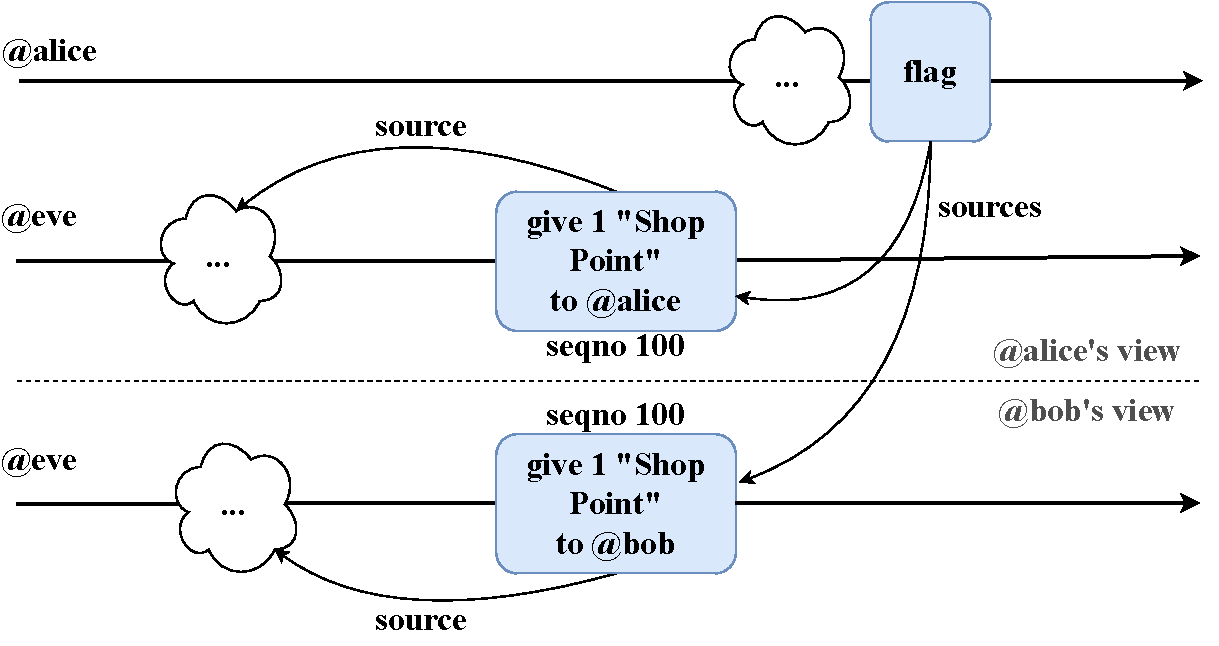
\includegraphics[width=0.45\textwidth]{figures/fork-double-spend}
\caption{Fork-based Double-Spending}
\end{figure}



\section{Applications}
\label{section:applications}

In this section, we present a large variety of applications that can be implemented with \ssbtokens to show the generality of our design.

\subsection{Fidelity Card}

A sandwich shop offers free sandwiches to customers once they have bought 10 sandwiches. 

Figure~\ref{figure:example} shows how the transactions happen. The yellow boxes represent events happening in the real world, while the blue boxes represent messages recorded on the logs, respectively of the shop owner (\textit{@shop}) and a regular customer (\textit{@customer}). In this example, the shop owner, in addition to giving a sandwich in exchange for $5$ Euros, also \textit{creates} then \textit{gives} a "Shop Point" to the customer. Once the customer has received 10 "Shop Points", she transfers the points to the shop owner to obtain a free sandwich. The shop owner then \textit{burns} the points, as the underlying promise of a free sandwidch has been redeemed.

\begin{figure}[htb]
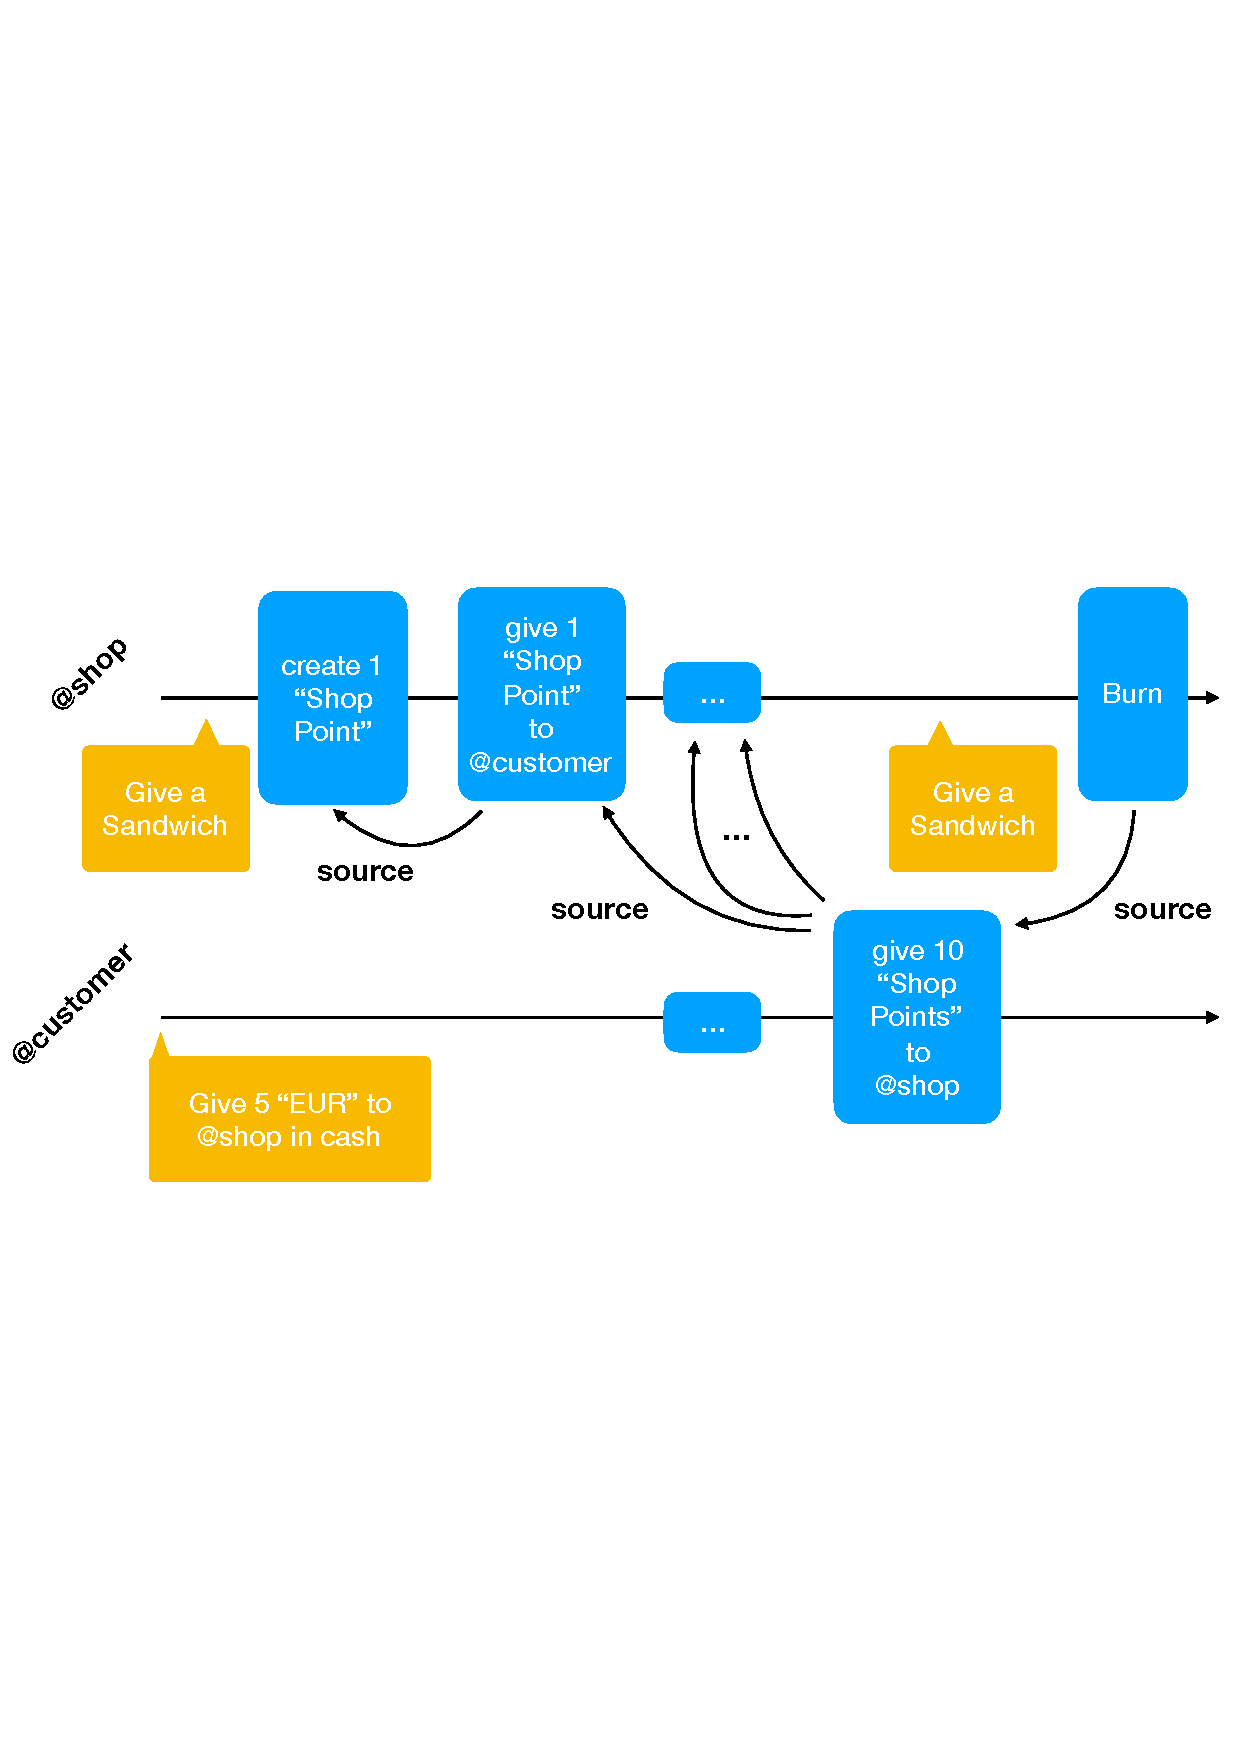
\includegraphics[width=0.40\textwidth]{./figures/example}
\caption{Example of \ssbtokens operations on SSB logs.}
\label{figure:example}
\end{figure}

\subsection{Tracking and Rewarding Open Source Contributions}

An open source maintainer creates tokens representing the number of hours volunteers have spent helping improve documentation, report and triage issues, submit patches for code improvements, etc. After validating the contributions, they create the required number of tokens and give them to volunteers. If or once a project receives money from donators, a "buy-back" program can distribute the money by allowing volunteers to exchange their contribution tokens for money at a fixed rate and up to a certain limit, possibly following the ratio of their total contributions compared to other volunteers.

\subsection{Community Crowdfunding}

A project initiator creates tokens that represent the future services that they plan to offer to the community, such as rides on a renovated sailboat.\footnote{This actually happened in the SSB community, albeit without proper token support.} Each token represent a certain amount of value, e.g. "1 day and night on the sailboat" or "10 Euros" of hosting/sailing services. The initiator sells their tokens to their community in exchange for other currencies or resources to carry the task. Once the sailboat is put in service, community members can exchange their tokens for the promised service. Alternatively, even before the project is actually completed, they can exchange them with other community members, for example, if they do not think they will need the services anymore.

\subsection{Token-supported Mesh Storage and Retransmission}

Tokens can be used to incentivize participation of nodes in a mesh of wireless nodes each implementing an SSB-compatible protocol. The tokens are used to compensate  costs incurred to store messages in transit and transmitting them to other nodes. Tokens can be emitted by each node independently and therefore represent a promise from a specific node that it will carry traffic in the future. Nodes can "pay" for storage and transmission using tokens created by themselves or by transferring back to other nodes the tokens they themselves created. Nodes individually accept tokens from any other node up to a limit after which traffic is not carried anymore, until the other nodes accept carrying traffic, paid with their own tokens, or they start paying for traffic using other nodes' tokens (obtained also after carrying traffic). In effect, this scheme implements a mutual credit system, including credit limitations.

A second alternative is to have one or multiple external parties, not participating in the mesh, creating tokens with which to pay for traffic. Nodes accept to carry traffic in exchange for those tokens and users of the mesh, source and/or destination for packets, can pay for delivery of traffic of specific logs by paying the nodes on one or multiple paths between the users. Because all transactions of tokens ultimately reference creation messages that only the token creators can sign, nodes cannot forge new tokens.

\section{Evaluation}
\label{section:evaluation}

In this section, we measure the resource consumption of \ssbtokens on affordable hardware to show that our design and implementation can be deployed on a large variety of devices, taking Raspberry Pis as representatives of the lower end of the scale. We use public traces of transactions from Ethereum application-specific (ERC) tokens implemented by smart contracts to show that our implementation can support a similar scale of users and number of transactions.

\subsection{Setup}

Ethereum ERC dataset size

\subsection{Storage}
\label{section:storage}

bytes per transaction
transactions per user (distribution)
total storage use

Number of users supported on common devices.

\subsection{CPU}

verification time per transaction (distribution)

\section{Related Work}
\label{section:related-work}

In this section, we present work that inspired our design and is related in its objectives and implementation techniques.

\textbf{Producer Credits} as proposed by Paul Grignon was a major inspiration for the design of \ssbtokens. No artificial scarcity. No need for community consensus to start using them, individual economic actors can introduce their own tokens for the community they interact with.

\textbf{Local Currencies}

\textbf{Crypto-currencies and Smart-Contracts} In contrast to Bitcoin and Ethereum, our implementation works with intermittent local connectivity, does not require solving cryptographic challenges (proof-of-work) or providing capital as collateral (proof-of-stake). Transactions between independent parties happen fully in parallel and total validation time is proportional to depth of transaction dependencies, which in all common cases is significantly faster than proof-of-work and proof-of-stake. Moreover, transaction latency is only proportional to the depth of previously unvalidated transactions since the validation of previous transactions is cached.


\textbf{TrustChain} Trust-based probabilisitic verification.  In contrast to other designs such as TrustChain~\ref{otte2020trustchain}, the \textit{give} operation of \ssbtokens  does not require confirmation by the recipient to accept the tokens. This removes the need for an out-of-band synchronization protocol but may result in users receiving unwanted tokens. In the latter case, they can block the sender or burn the tokens.


\textbf{Witness-based Validation} Crypto-currency consensus number.

Helium people-powered network \url{helium.com}

Nuglets \url{https://infoscience.epfl.ch/record/52377}

Hal Varian \url{https://scholar.google.com/citations?user=WbYQGjcAAAAJ&hl=en&oi=ao}

\textbf{Token-supported Mesh} Nuglets~\cite{buttyan2001nuglets} also uses tokens to retribute mesh network nodes for their services. In contrast to Nuglets however, using \ssbtokens enables each node to emit tokens for their own services and individually choose whose other nodes' tokens (and associated traffic) they are going to accept and up to which limit. In Nuglets, token transfers are performed in a secure environment to prevent nodes from creating tokens and free-riding on the services offered by other nodes. With \ssbtokens, nodes instead only create tokens for services that they themselves provide. Moreover, nodes cannot create tokens for other nodes, they can only give or burn those they have received. There is therefore no need for a secure environment to update token holdings. 
%The use of \ssbtokens is also compatible with token creation by an external entity not participating in the mesh routing, as long as the participating nodes are wiling to accept external tokens, while still guaranteeing participating nodes cannot forge similar tokens.

\textbf{Non-Fungible Tokens} Our system trivially supports recording NFTs transactions. To create a new one an author, presumably from a reputable organization, simply has to create a new token in its log and mention in the token description the corresponding asset it represents. Other users that want to trade NFTs create SSB identities and give them to each other.

\section{Conclusion and Future Work}
\label{section:conclusion}

At scale, requires an exchange service to conveniently convert one token type to another.

Integration of tokens with replication operations.

Adding witness support for really valuable transactions.






\bibliographystyle{ACM-Reference-Format}
\bibliography{main}

\appendix

\section{Definitions}

\definition{\textit{Store}: Local database of all SSB logs replicated by a node.}

\definition{\textit{Author}: SSB log in which an operation is recorded.}

\definition{\textit{Log ancestor}: operation that appears before another operation, in the log the same author.}

\definition{\textit{Ancestor operation}: recorded token operation used as source for a subsequent token operation. Might be in a different log.}

\definition{\textit{Root operation}: earliest transitive ancestor operation of a token operation. Must be a \texttt{tokens/create} message.}

\definition{\textit{Owner}: current holder of tokens, i.e. author of a \texttt{tokens/create} message or \textit{recipient} of a \texttt{tokens/give} message.}


\section{List of Anticipated Potential Attacks and Responses}

\begin{itemize}
	\item Creating operations with wrong token hashes, to show up in other people balances. -> Ruled out by computing the balance only on valid messages.
\end{itemize}



\section{Open Questions}

\begin{itemize}
\item Empirical evidence (with simulation?) for scaling limit? (I am making the hypothesis that it should work 
\end{itemize}

\end{document}